\qquad Os Gráficos \ref{fig:geral_crescente} e \ref{fig:geral_decrescente}
apresentam, respectivamente, o tempo de execução dos cinco algoritmos
estudados neste trabalho para entradas já ordenadas (crescente) e para
entradas em ordem decrescente (o cenário mais desfavorável para o
Insertion e o Bubble Sort), permitindo comparar diretamente o desempenho
de Insertion Sort, Selection Sort, Bubble Sort, Shell Sort e Merge Sort.
Ambos utilizam escala logarítmica nos dois eixos, necessária porque os
tempos variam de microssegundos a centenas de segundos. Valores iguais
a zero (tempos menores que a resolução do relógio, de cerca de 1
$\mu$s nestas medições) não podem ser representados em escala
logarítmica; o único caso neste trabalho é o do Bubble Sort com 1.000
elementos em entrada crescente, que por isso aparece como uma
interrupção na curva do Bubble Sort no Gráfico \ref{fig:geral_crescente}.

\begin{figure}[htbp]
    \centering
    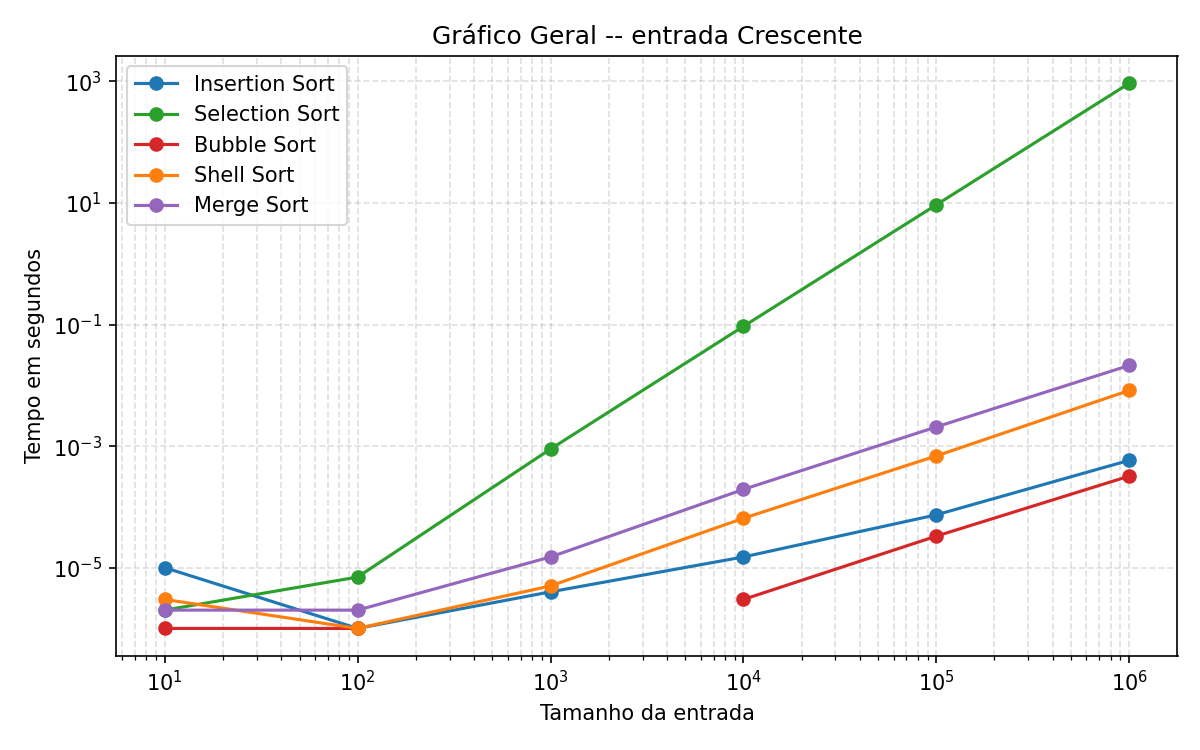
\includegraphics[width=14cm]{Imagens/Geral/grafico_geral_crescente_log.png}
    \caption{Gráfico geral (escala logarítmica) -- entrada crescente}
    \label{fig:geral_crescente}
\end{figure}

\begin{figure}[htbp]
    \centering
    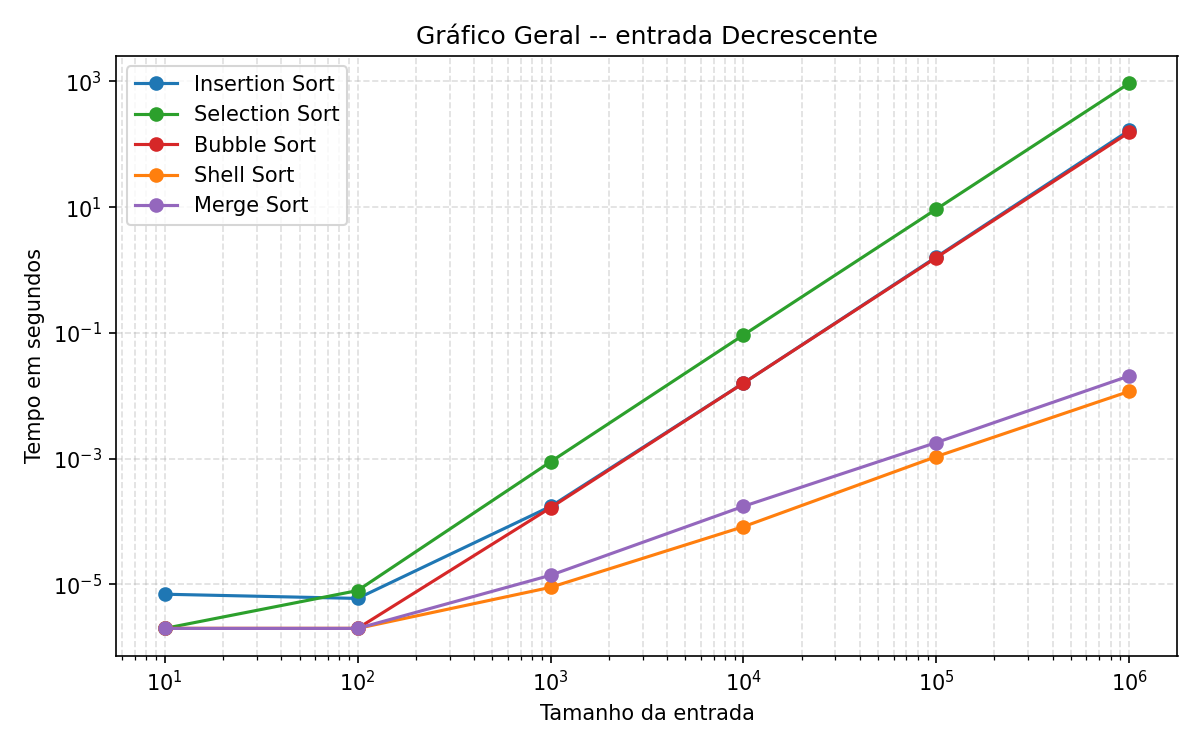
\includegraphics[width=14cm]{Imagens/Geral/grafico_geral_decrescente_log.png}
    \caption{Gráfico geral (escala logarítmica) -- entrada decrescente}
    \label{fig:geral_decrescente}
\end{figure}

\qquad Na entrada crescente (Gráfico \ref{fig:geral_crescente}) os
algoritmos se separam em três grupos: o Insertion e o Bubble Sort, que
têm desempenho linear nesse cenário e levaram menos de um milésimo de
segundo para 1.000.000 de elementos; o Shell Sort e o Merge Sort, da
ordem de $n \log n$, com 0,008 s e 0,021 s; e o Selection Sort, que
continua quadrático (934,9 s) por não se beneficiar da ordenação
prévia. Na entrada decrescente (Gráfico \ref{fig:geral_decrescente}) a
separação é em dois grupos: os três algoritmos quadráticos
(Selection Sort com 937,3 s, e Insertion e Bubble Sort com cerca de
160 s, com curvas praticamente sobrepostas) e, cerca de quatro ordens
de grandeza abaixo, o Shell Sort (0,012 s) e o Merge Sort (0,021 s).
